% !TeX program = xelatex
% !TeX encoding = UTF-8
% ============================================================
%  第二十七届华南大学生物理实验设计大赛 命题类作品研究报告
%  《刻线之间见星河——光栅衍射背后的国之重器》
%  由 213.docx 自动转换生成（编译方式: xelatex）
% ============================================================
\documentclass[12pt,a4paper]{ctexrep}

% ---- 章节标题格式(一级标题编号 1,2,3...) ----
\ctexset{
  chapter = {
    name = {},
    number = \arabic{chapter},
    format = \centering\zihao{3}\heiti,
    titleformat = \centering\zihao{3}\heiti,
    beforeskip = 10pt,
    afterskip = 24pt,
  },
  section = {
    format = \zihao{4}\heiti,
    beforeskip = 18pt,
    afterskip = 10pt,
  },
  subsection = {
    format = \zihao{-4}\heiti,
    beforeskip = 14pt,
    afterskip = 8pt,
  },
}

% ---- 页面设置 (与原 Word 文档页边距一致) ----
\usepackage[top=1in,bottom=1in,left=1.25in,right=1.25in]{geometry}

% ---- 数学与公式 ----
\usepackage{amsmath}
\usepackage{amssymb}

% ---- 图片 / 表格 / 图表标题 ----
\usepackage{graphicx}
\graphicspath{{figures/}}
\usepackage{booktabs}
\usepackage{array}
\usepackage{caption}
\usepackage[font=small]{subcaption}

% ---- 列表 ----
\usepackage{enumitem}

% ---- 公式与浮动体间距(全文统一) ----
\setlength{\abovedisplayskip}{8pt plus 2pt minus 2pt}
\setlength{\belowdisplayskip}{8pt plus 2pt minus 2pt}
\setlength{\abovedisplayshortskip}{4pt plus 1pt minus 1pt}
\setlength{\belowdisplayshortskip}{4pt plus 1pt minus 1pt}
\setlength{\intextsep}{10pt plus 2pt minus 2pt}
\setlength{\textfloatsep}{12pt plus 2pt minus 2pt}
\setlength{\floatsep}{10pt plus 2pt minus 2pt}

% ---- 代码 ----
\usepackage{xcolor}
\usepackage{listings}
\lstdefinestyle{pycode}{
  language=Python,
  basicstyle=\ttfamily\footnotesize,
  keywordstyle=\color{blue!70!black},
  commentstyle=\color{green!45!black},
  stringstyle=\color{red!60!black},
  showstringspaces=false,
  breaklines=true,
  breakatwhitespace=false,
  columns=fullflexible,
  keepspaces=true,
  backgroundcolor=\color{gray!12},
  frame=single,
  framesep=4pt,
  xleftmargin=4pt,
  xrightmargin=4pt,
  numbers=left,
  numberstyle=\tiny\color{gray},
}
\lstset{style=pycode}

% ---- 下划线(标题页) ----
\usepackage[normalem]{ulem}

% ---- 超链接 ----
\usepackage[hidelinks]{hyperref}

% ---- 中文字体与段落 ----
\setlength{\parindent}{2em}
\usepackage{indentfirst}
\linespread{1.2}

% ---- 等宽字体 ----
% 代码注释/字符串中含希腊字母(λ θ π 等), 默认 Latin Modern Mono 无对应字形,
% 改用 Windows 自带 Consolas(覆盖希腊字母及上下标符号)
\setmonofont{Consolas}

% ---- 正文裸希腊字母 ----
% 正文中直接出现的希腊字母(如 "波长 λ"、"衍射角 θ")由中文字体渲染,
% Latin Modern Roman 无希腊字形
\xeCJKDeclareCharClass{CJK}{"03B1 -> "03C9, "03D1, "03D5, "03D6, "03F0, "03F1}

% ---- 参考资料标题 ----
% 正文改用 \cite 后, 参考资料列表由 thebibliography 自动生成标题
\renewcommand{\bibname}{参考资料}

\begin{document}

\begin{titlepage}
\begin{center}
\vspace*{1.5cm}
{\zihao{3}\heiti 第二十七届华南大学生物理实验设计大赛\par}
\vspace{0.8cm}
{\zihao{3}\heiti 命题类作品\par}
\vspace{0.8cm}
{\fontsize{48pt}{58pt}\selectfont\bfseries 研究报告\par}
\vspace{1cm}
\vspace{2.5cm}
{\zihao{3} 赛道：\underline{大学物理理论课辅助教学微视频}\par}
\vspace{1.2cm}
{\zihao{3} 课题：\underline{光栅衍射}\par}
\vspace{1.2cm}
\vfill
{\zihao{3} 2026年8月28日\par}
\end{center}
\end{titlepage}

\chapter*{摘要}
\addcontentsline{toc}{chapter}{摘要}

本项目围绕大学物理理论课中的光栅衍射主题，融合理论分析、数值仿真与微视频制作，系统阐述了从单缝衍射、多缝干涉到光栅衍射的完整物理图像。理论层面，以惠更斯-菲涅耳原理为出发点，推导单缝夫琅禾费衍射与多缝干涉的光强分布公式，进而得到光栅衍射总光强公式，重点剖析缺级现象、亮纹半角宽度与色分辨本领等核心特性。仿真层面，基于 Python 科学计算生态（NumPy、Matplotlib）对单缝衍射、多缝干涉、光栅缺级及色分辨本领进行数值模拟，并结合 Manim 动画引擎与 Blender 三维渲染技术，将抽象的矢量叠加与光强分布过程转化为直观的动态画面。在此基础上制作完成约 3 分钟的科普微视频，以「大国重器悬念引入—原理拆解—特性分析—应用升华」的叙事结构，将光栅衍射原理与光刻机、郭守敬望远镜（LAMOST）等国家重大科技工程相结合，并配套开发可参数调节的交互式仿真网页。项目实现了理论、仿真、动画与实验素材的有机融合，为大学物理理论课辅助教学提供了一套集科学性、直观性与趣味性于一体的微视频教学资源。

\noindent 关键词：\textbf{光栅衍射；夫琅禾费衍射；缺级现象；色分辨本领；微视频教学}

\tableofcontents

\chapter{项目概述}

\section{项目背景}

光栅衍射是波动光学的核心知识点，也是现代精密光学工程的物理基础。从芯片制造核心的 EUV 光刻机，到大视场光谱巡天的郭守敬望远镜，再到可控核聚变 “人造太阳” 的光谱诊断系统，光栅器件的性能直接决定了高端制造与前沿科研的精度上限。

在传统大学物理教学与大众科普中，光栅衍射长期存在 “原理抽象、理解困难” 的痛点：一方面，单缝衍射、多缝干涉、缺级现象等知识点涉及复杂的矢量叠加与数学推导，仅靠静态公式与示意图难以建立直观的物理图像；另一方面，多数科普内容仅停留在理论讲解层面，未能将基础原理与大国重器的工程应用建立关联，难以让受众感知物理知识的现实价值。

伴随短视频与新媒体科普的快速发展，受众对科学内容的可视化、故事化、互动化需求持续提升。以动画微视频为载体，将抽象的光学原理转化为直观的动态演示，同时结合前沿科技应用场景，成为提升物理科普效果与教学效率的重要方向。本项目正是基于这一背景，围绕光栅衍射主题开发系统化的科普微视频作品。

\section{项目简介}

本项目以 “光栅衍射” 为核心主题，制作时长约 3 分钟的科普微视频，同时配套开发可交互的光栅衍射仿真体验工具。

项目以波动光学理论为学术基础，遵循 “现象引入 — 原理拆解 — 特性分析 — 应用升华” 的认知逻辑，系统讲解惠更斯-菲涅耳原理、单缝夫琅禾费衍射、多缝干涉、光栅衍射缺级、半角宽度与色分辨本领等核心知识点。视频融合三维光场动画、二维光路推导、实拍素材与前沿工程案例，将抽象的数学物理过程转化为可视化的动态画面，降低理解门槛。

项目核心产出包括：1 支完整的光栅衍射科普微视频、全套原理动画素材、1 个可参数调节的光栅衍射互动网页。作品既可以作为大学物理实验的辅助教学资源，也可以作为面向大众的精密光学科普内容，帮助受众理解光栅技术的科学价值，感知我国在高端光学领域的技术突破。

\chapter{基本理论}

\section{惠更斯-菲涅耳原理}

惠更斯-菲涅耳原理是研究衍射现象的理论基础，其核心思想可以表述为：\textbf{波前上的每一个面元都可以看作是发射子波的波源，空间中任意一点的光振动，是所有这些子波在该点的相干叠加}。

惠更斯最早提出‘子波’的概念，能定性说明波绕过障碍物的传播方向（即衍射现象），但无法解释衍射图样的光强分布。菲涅耳在此基础上补充了‘子波相干叠加’的假设，认为各子波在空间相遇时产生干涉效应，空间某点的光振动由所有子波在该点的振幅与相位相干叠加决定。其数学表达式为：

% 原文档此处为公式图片 image1.png, 已重建为 LaTeX 公式(请对照原文核对)
\begin{equation*}
U(P)=C\oint_{\Sigma}U(Q)\,\frac{e^{ikr}}{r}\,K(\theta)\,\mathrm{d}\sigma
\end{equation*}

\noindent 式中：$U(P)$ 为空间场点 $P$ 的复振幅；$U(Q)$ 为波前上某点 $Q$（次级波源）处的波扰；$C$ 为比例常数；$K(\theta)$ 为倾斜因子，描述子波振幅随衍射角 $\theta$ 的变化规律；$\mathrm{d}\sigma$ 为波前 $\Sigma$ 上的面元；$r$ 为面元到场点 $P$ 的距离；$k$ 为波数，$k=\frac{2\pi}{\lambda}$。

该原理表明，一切波传播的现象可以用无穷多子波的叠加来解释，于是光栅衍射现象可以通过子波相干叠加的思想进行分析与计算。

\section{夫琅禾费衍射基础}

根据光源、衍射屏、接收屏三者的相对位置，衍射通常分为两大类：菲涅耳衍射（近场衍射）与夫琅禾费衍射（远场衍射）。

\textbf{菲涅耳衍射}：光源和接收屏（或其中之一）距离衍射屏为有限远，入射波与衍射波均为球面波，计算相对复杂。

\textbf{夫琅禾费衍射}：光源和接收屏都距离衍射屏无穷远，入射光与衍射光均为平行光，与菲涅耳衍射的远场近似。在实际实验中，通常借助两个透镜实现：第一个透镜将点光源发出的光转化为平行光入射到衍射屏，第二个透镜将衍射后的平行光会聚到焦平面上进行观察。

夫琅禾费衍射的近似条件为：衍射屏到场点的距离 $z$ 满足 $z\gg\frac{{a}^{2}}{\lambda}$，其中 $a$ 为衍射孔的线度，$\lambda$ 为入射光波长。在该近似下，衍射积分的计算可以大幅简化，同时衍射图样的相对强度分布不随传播距离变化，整体几何尺寸与距离 $z$ 成正比，具有稳定的分布规律。

夫琅禾费衍射是光栅光谱仪的核心工作模式，也是光刻机等光学仪器投影成像的基础理论框架之一，本项目将以此为重点讲解衍射类型。

\section{单缝夫琅禾费衍射}

单缝夫琅禾费衍射是研究光栅衍射的基础。设狭缝宽度为 $a$，波长为 $\lambda$ 的平行光垂直入射，衍射角为 $\theta$ 的平行光经透镜会聚到焦平面上。

\subsection{物理过程}

将狭缝处的波前沿缝宽方向分割为无穷多个等宽的子波源，每个子波源向各个方向发射子波。衍射角为 $\theta$ 的一组平行光，从波前不同位置出发时存在光程差，到达接收屏同一点时具有不同的相位，通过相干叠加形成最终的光强分布。

\subsection{光强公式推导}

通过衍射积分计算可得，单缝夫琅禾费衍射的光强分布为：

\begin{equation*}
I={I}_{0}{\left( \frac{\sin{\alpha}}{\alpha} \right)}^{2}
\end{equation*}

式中：${I}_{0}$ 为中央主极大的光强；$\alpha$ 为单缝衍射的相位参数，其物理意义是狭缝边缘与中心的子波在衍射角 $\theta$ 方向的相位差的一半，表达式为：

\begin{equation*}
\alpha=\frac{\pi a\sin \theta}{\lambda}
\end{equation*}

\subsection{衍射图样特征}

\begin{enumerate}[label=\arabic*., leftmargin=2em, itemsep=0pt]
\item \textbf{主极大位置}：当 $\alpha=0$（即 $\theta=0$）时，$\frac{\sin{\alpha}}{\alpha}=1$，光强取得最大值 ${I}_{0}$，对应中央亮纹，能量主要集中在中央亮纹内。
\item \textbf{极小值位置}：当 $\alpha=\pm k\pi$（$k=1,2,3\cdots$），即 $a\sin \theta=\pm k\lambda$ 时，光强为 0，对应暗纹位置。
\item \textbf{次级大}：相邻两个暗纹之间存在一个次极大，位置满足 $\tan \alpha=\alpha$，其光强随级次增大迅速衰减，第一级次极大光强仅为中央主极大的约 4.7\%。
\item \textbf{条纹宽度}：中央亮纹的角宽度为两侧第一级暗纹的夹角，$\Delta{\theta}_{0}=\frac{2\lambda}{a}$；其他各级亮纹的角宽度为中央亮纹的一半，$\Delta\theta=\frac{\lambda}{a}$。缝宽越小，衍射效应越显著，条纹越宽。
\end{enumerate}

\section{多缝干涉原理}

光栅由大量等宽、等间距的平行狭缝组成，设缝数为 $N$，相邻两缝的中心间距为 $d$（称为光栅常数）。分析多缝干涉时，先忽略单缝衍射的调制作用，将每条狭缝近似为一个点波源。

\subsection{相位差与光强分布}

相邻两缝发出的衍射角为 $\theta$ 的平行光，到达接收屏同一点的光程差为 $d\sin \theta$，对应的相位差为：

\begin{equation*}
\delta=\frac{2\pi}{\lambda}d\sin \theta
\end{equation*}

令 $\beta=\frac{\delta}{2}=\frac{\pi d\sin \theta}{\lambda}$，即相邻两束光相位差的一半。

将 $N$ 个缝的光振动用矢量表示，通过矢量叠加法或复振幅求和，可推导出多缝干涉的光强分布：

\begin{equation*}
I={I}_{1}{\left( \frac{\sin N\beta}{\sin{\beta}} \right)}^{2}
\end{equation*}

式中：${I}_{1}$ 为单条缝在该方向的光强。

\subsection{干涉主极大与光栅方程}

当相邻两缝的光程差为波长的整数倍，即 $d\sin \theta=k\lambda$（$k=0,\pm1,\pm2,\cdots$）时，$\beta=k\pi$，此时 $\frac{\sin N\beta}{\sin{\beta}}=N$，所有缝的光振动同相位，总振幅为单缝的 $N$ 倍，总光强为单缝的 ${N}^{2}$ 倍，光强达到峰值，称为\textbf{干涉主极大}。

公式 $d\sin \theta=k\lambda$ 即为\textbf{光栅方程}，是光栅最核心的规律。它表明不同波长的光对应不同的衍射角，这是光栅能够分光的物理基础。

\subsection{干涉图样特征}

\begin{itemize}[leftmargin=2em, itemsep=2pt]
\item 主极大条纹细锐明亮，光强远高于次极大；
\item 两个相邻主极大之间，分布着 $N-1$ 条暗纹和 $N-2$ 个次极大；
\item 缝数 $N$ 越大，主极大条纹越细越亮，背景越暗，分光效果越好。
\end{itemize}

\section{光栅衍射与缺级现象}

实际的光栅衍射是单缝衍射效应与多缝干涉效应的共同结果：单缝衍射对各个方向的光强进行调制，多缝干涉决定主极大的位置与精细结构。

\subsection{光栅衍射总光强}

将单缝衍射因子与多缝干涉因子相乘，得到光栅衍射的总光强分布：

\begin{equation*}
I={I}_{0}{\left( \frac{\sin{\alpha}}{\alpha} \right)}^{2}{\left( \frac{\sin N\beta}{\sin{\beta}} \right)}^{2}
\end{equation*}

式中：$\alpha=\frac{\pi a\sin\theta}{\lambda}$，$\beta=\frac{\pi d\sin\theta}{\lambda}$。

\subsection{缺级现象的成因}

如果某一级干涉主极大的位置，恰好与单缝衍射的极小值位置重合，那么该级主极大的光强会被调制为 0，对应的亮纹完全消失，这种现象称为\textbf{缺级}。

缺级满足的条件为：

% 原文档此处为公式图片 image3.png, 已重建为 LaTeX 公式(请对照原文核对)
\begin{equation*}
d\sin\theta=k\lambda,\qquad a\sin\theta=k'\lambda
\end{equation*}

联立两式可推导出缺级级次公式：

\begin{equation*}
k=\frac{d}{a}k'\qquad(k'=\pm1,\pm2,\pm3,\cdots)
\end{equation*}

当光栅常数与单缝缝宽的比值为整数时，对应整数倍衍射级次会全部消失。缺级现象直观证明了光栅衍射是「单缝衍射包络调制多缝干涉条纹」的复合光学现象，是光栅衍射区别于单纯多缝干涉的核心特征。

\section{光栅半角宽度与色分辨本领}

\subsection{半角宽度}

光栅衍射主极大亮纹并非理想几何线条，具备一定角宽度，工程与光学教学中统一使用\textbf{半角宽度}定量描述亮纹精细度：定义为衍射主极大中心位置到相邻第一级暗纹的角距离。

根据光栅暗纹条件与光栅方程微分推导，第 $k$ 级主极大半角宽度公式为：

% 原文档此处为公式图片 image5.GIF, 已重建为 LaTeX 公式(请对照原文核对)
\begin{equation*}
\Delta\theta_k=\frac{\lambda}{Nd\cos\theta_k}
\end{equation*}

式中：$N$ 为光栅总刻缝数，$d$ 为光栅常数，$\theta_k$ 为第 $k$ 级衍射角。由公式可得核心规律：光栅总缝数 N 越大，半角宽度越小，衍射亮纹越锐利、背景暗区越干净，分光精度越高。这也是高精度光学光栅均采用高密度、多刻线设计的理论依据。

\subsection{色分辨本领}

光栅的核心工程价值为分光能力，能够区分波长极接近的复合光谱，该性能指标定义为\textbf{色分辨本领}。行业与物理教学统一采用\textbf{瑞利判据}作为分辨临界标准：一条谱线的主极大峰值恰好落在相邻谱线的第一级暗纹位置时，认定两条谱线刚好可分辨。

设可分辨的最小波长差为$\delta\lambda$，中心波长为 $\lambda$，联立光栅方程与半角宽度公式，推导出光栅色分辨本领公式：

% 原文档此处为公式图片 image9.GIF, 已重建为 LaTeX 公式(请对照原文核对)
\begin{equation*}
R=\frac{\lambda}{\delta\lambda}=kN
\end{equation*}

该公式表明：光栅分辨本领仅由\textbf{衍射级次 $k$} 和\textbf{总刻缝数 $N$} 决定，与光栅常数无关。在实际工程应用中，提升光谱分辨精度的核心手段为：选用更高衍射级次、增加光栅有效刻线总数，这也是郭守敬望远镜、高端光刻机光栅系统的核心设计逻辑。

\chapter{实验与仿真设计}

\section{光栅衍射仿真设计}

\subsection{仿真目的}

本项目依托数值仿真技术，对单缝衍射、多缝干涉、光栅缺级、亮纹半角宽度及色分辨本领等一系列核心光学现象进行精准复现。通过系统性的参数调控，直观验证理论公式的内在规律，为科普视频动画的制作提供精准、可量化且来源清晰的物理数据，从源头上规避纯手绘动画可能造成的物理失真，确保科普内容的科学性与严谨性。

\subsection{仿真工具与环境}

仿真以 Python 科学计算生态为核心，并辅以专业光学计算软件进行数据交叉校验。具体工具链配置如下：采用 NumPy 库执行数值计算，Matplotlib 库完成可视化绘图；引入 Mathematica 进行公式推导验证及高精度曲线拟合。该仿真环境运行稳定，计算精度满足光学科普与教学应用需求，所输出的图像、曲线及帧序列均可直接用于视频渲染合成。仿真代码界面如图~\ref{fig:code}所示。

\begin{figure}[htbp]
\centering
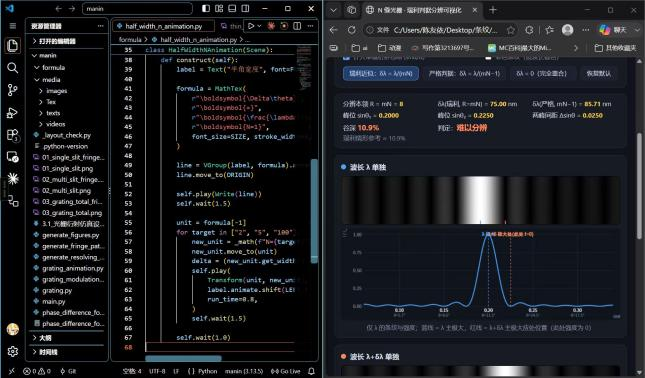
\includegraphics[width=0.9\textwidth]{figures/image10.jpeg}
\caption{仿真代码界面（Python 数值仿真）}
\label{fig:code}
\end{figure}

\subsection{仿真参数设置}

为简化，并保证不同工况间的数值可比性，仿真统一采用归一化波长 $\lambda=1.0$，以 $\sin\theta$ 作为衍射角采样变量并覆盖 $[-1,\,1]$ 全域，确保正负各级衍射图样完整呈现。可变核心参数包括单缝缝宽 $a$、光栅常数 $d$ 与光栅总缝数 $N$。基准工况取 $a=3.0$、$d=12.0$、$N=6$，对应 $d/a=4$，此时每第 4 级干涉主极大恰与单缝衍射包络零点重合而发生缺级，调制结构清晰可辨。在此基础上另设多组对照工况，如 $d/a=3,4,6,8,12$ 与衍射级次 $k=1,2,3,5,8$，分别考察缺级规律、亮纹半角宽度及色分辨本领随参数的变化。

\subsection{仿真流程与方案}

光栅衍射总光强由单缝衍射因子与多缝干涉因子逐点相乘得到，两因子均为 $\sin(\cdot)/(\cdot)$ 型超越函数\cite{ref2}。主极大位置、缺级级次与亮纹半角宽度取决于两因子在全衍射角域内的相对取值，解析方法只能给出零级、主极大等若干特例结论。为此本节采用数值采样方案\cite{ref7}，依「理论建模—算法实现—必要修正—结果验证」的顺序推进。

核心计算步骤如下：

\begin{enumerate}[label=(\arabic*), leftmargin=2.4em, itemsep=2pt]
\item \textbf{离散采样}：以 $\sin\theta$ 为采样变量，在 $[-1,\,1]$ 全域均匀取 4000 点，兼顾主极大锐度与计算量；
\item \textbf{逐点求解}：代入相位参数 $\alpha=\pi a\sin\theta/\lambda$、$\beta=\pi d\sin\theta/\lambda$，逐点计算两因子并相乘；
\item \textbf{峰值归一化}：按各工况自身峰值归一，消除缝数 $N$ 引入的 $N^{2}$ 亮度差异，使不同参数下的曲线可直接比较。
\end{enumerate}

上述公式在 $\alpha\to 0$ 与 $\sin\beta\to 0$ 处为 $0/0$ 型不定式，数值计算将返回无效值，需按极限关系予以修正\cite{ref4}：

\begin{equation*}
\lim_{\alpha\to 0}\left(\frac{\sin\alpha}{\alpha}\right)^{2}=1,
\qquad
\left(\frac{\sin N\beta}{\sin\beta}\right)^{2}=
\begin{cases}
N^{2}, & \beta=k\pi\\[2pt]
0, & \text{其他}
\end{cases}
\end{equation*}

第二处修正在于条纹图的灰度映射。单缝衍射次级极大不足主极大的 5\%，若按线性强度直接成像，包络调制后的高阶主极大几乎不可见；而多缝干涉各级主极大等亮，无需补偿。故仅对归一化强度施加 $\gamma$ 校正（单缝取 $\gamma=0.35$，总光强取 $\gamma=0.45$），压缩动态范围后次级结构方清晰可辨。

最后由结果验证闭环。色分辨本领以 $R=kN$ 为基准，并计入缺级的影响：当 $d/a$ 为整数时 $k=(d/a)k'$ 各级整级缺失，中央衍射极大内的最高可用级次降为 $k_{\max}=d/a-1$。据此计算可分辨的最小波长差 $\Delta\lambda=\lambda/R$，并与钠双线（589.0 nm 与 589.6 nm，$\lambda/\Delta\lambda\approx 982$）的分辨要求对照，验证了仿真结果的物理合理性。

\subsection{仿真输出成果}

完整输出五类仿真成果：单缝衍射光强分布与条纹图样、多缝干涉精细条纹、光栅衍射缺级对比图样、不同缝数下半角宽度变化动画、多组参数下色分辨本领对比曲线。所有成果严格贴合物理公式，保证科普视频的科学性与严谨性。主要数值仿真输出如图~\ref{fig:sim-output}所示，其中(a)为单缝衍射光强分布曲线，(b)为对应的二维衍射条纹图样，(c)(d)为多缝干涉因子的光强分布与条纹图样，(e)(f)为光栅衍射总光强分布与总图样，可清晰观察到单缝包络对干涉条纹的调制与缺级现象。色分辨本领随缝数的变化、考虑缺级后最高可用级次下的色分辨本领以及可分辨最小波长差随缝数的变化分别如图~\ref{fig:resolving-N}、图~\ref{fig:resolving-missing}与图~\ref{fig:resolving-dlambda}所示。

\begin{figure}[htbp]
\centering
\begin{subfigure}[b]{0.48\textwidth}
\centering
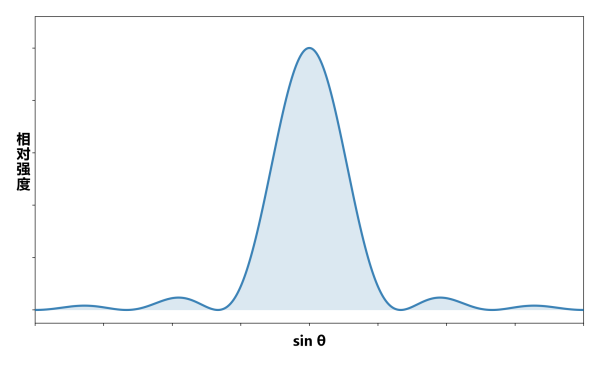
\includegraphics[width=\textwidth]{figures/image11.png}
\caption{单缝衍射光强分布}
\label{fig:sim-a}
\end{subfigure}
\hfill
\begin{subfigure}[b]{0.48\textwidth}
\centering

\includegraphics[width=\textwidth]{figures/image12.png}
\caption{单缝衍射图样}
\label{fig:sim-b}
\end{subfigure}
\hfill
\begin{subfigure}[b]{0.48\textwidth}
\centering
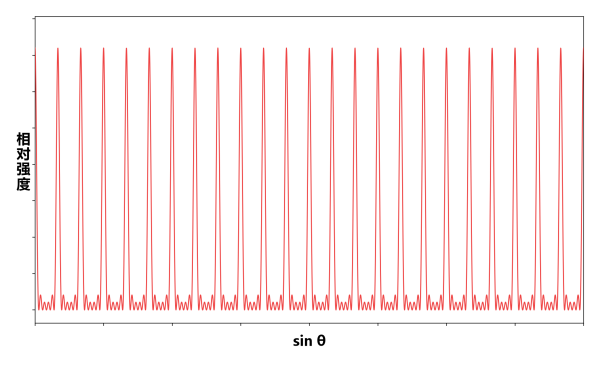
\includegraphics[width=\textwidth]{figures/image13.png}
\caption{多缝干涉因子光强分布}
\label{fig:sim-c}
\end{subfigure}
\hfill
\begin{subfigure}[b]{0.48\textwidth}
\centering
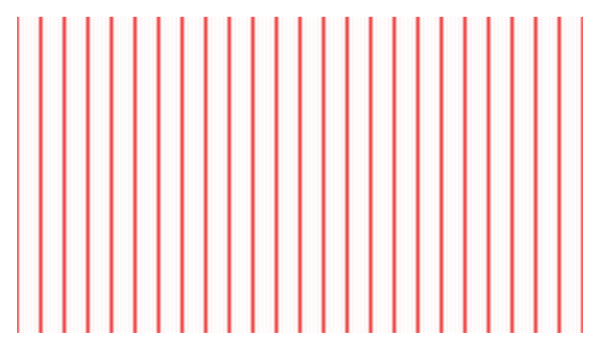
\includegraphics[width=\textwidth]{figures/image14.png}
\caption{多缝干涉因子图样}
\label{fig:sim-d}
\end{subfigure}
\hfill
\begin{subfigure}[b]{0.48\textwidth}
\centering
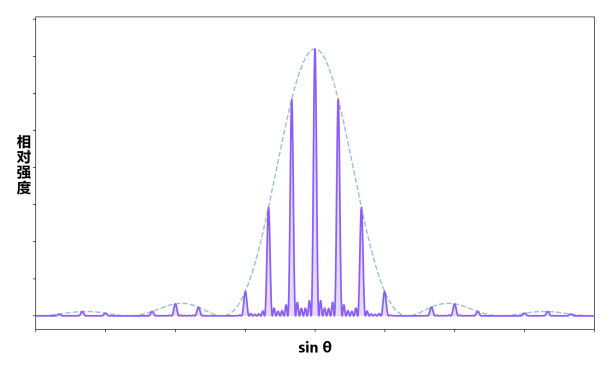
\includegraphics[width=\textwidth]{figures/image15.png}
\caption{光栅总光强分布}
\label{fig:sim-e}
\end{subfigure}
\hfill
\begin{subfigure}[b]{0.48\textwidth}
\centering
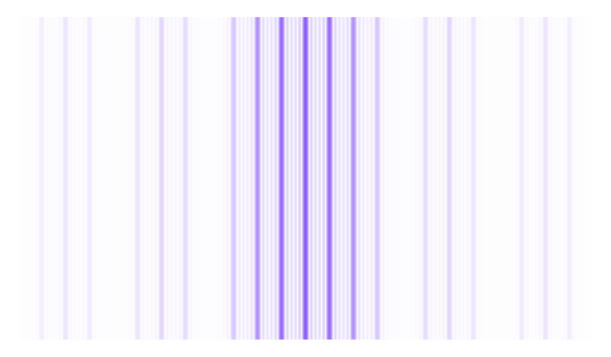
\includegraphics[width=\textwidth]{figures/image16.png}
\caption{光栅总图样}
\label{fig:sim-f}
\end{subfigure}

\caption{光栅衍射数值仿真输出成果}
\label{fig:sim-output}
\end{figure}

\begin{figure}[htbp]
\centering
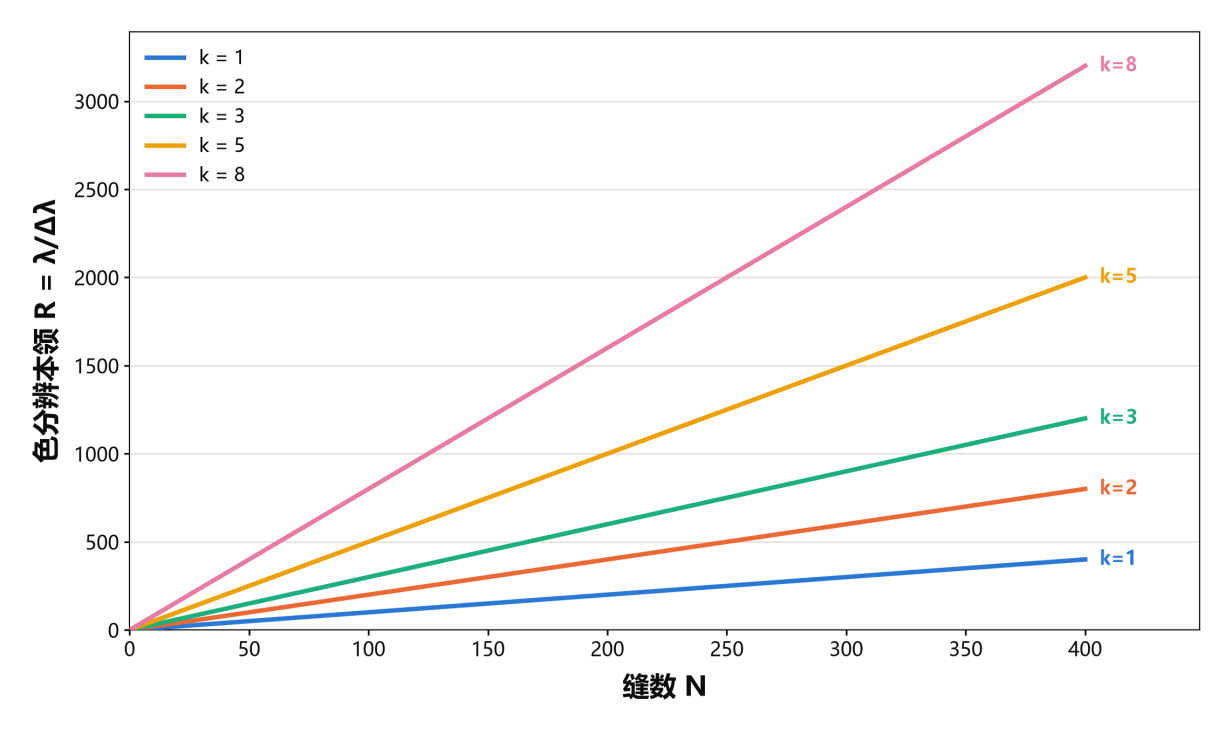
\includegraphics[width=0.9\textwidth]{figures/image17.png}
\caption{光栅色分辨本领随缝数的变化}
\label{fig:resolving-N}
\end{figure}

\begin{figure}[htbp]
\centering
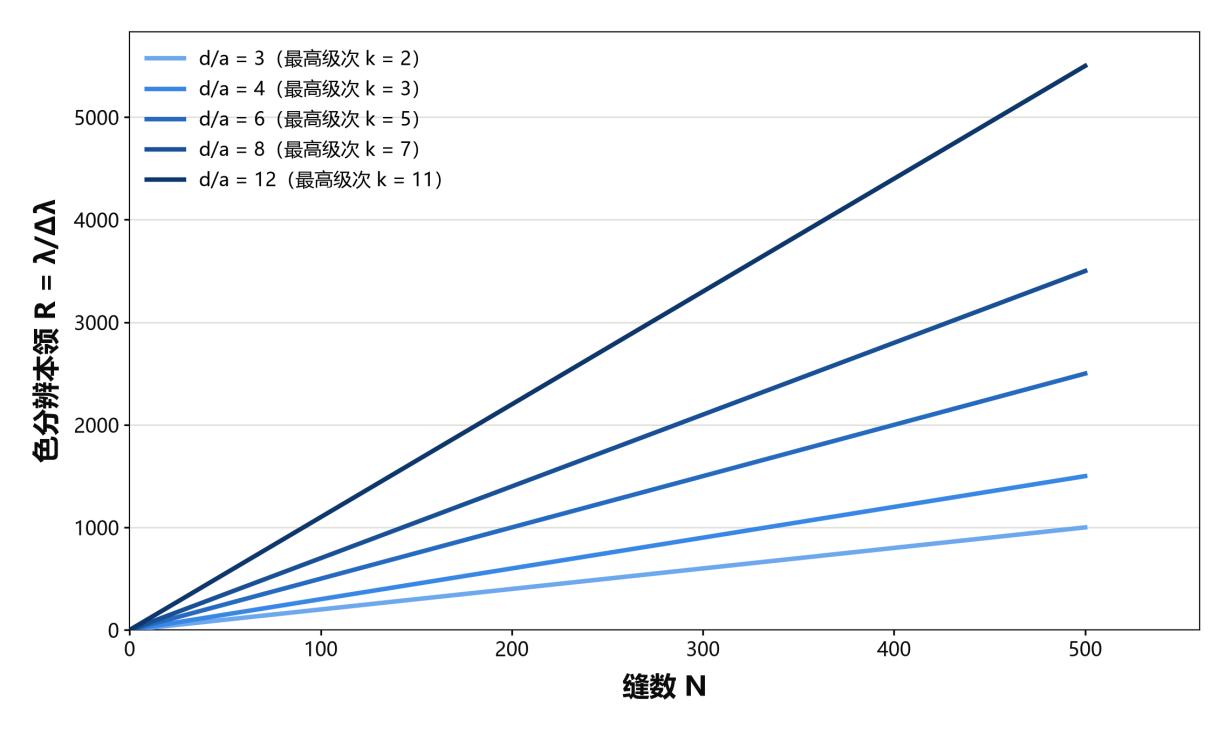
\includegraphics[width=0.9\textwidth]{figures/image18.png}
\caption{考虑缺级：最高可用级次下的色分辨本领}
\label{fig:resolving-missing}
\end{figure}

\begin{figure}[htbp]
\centering
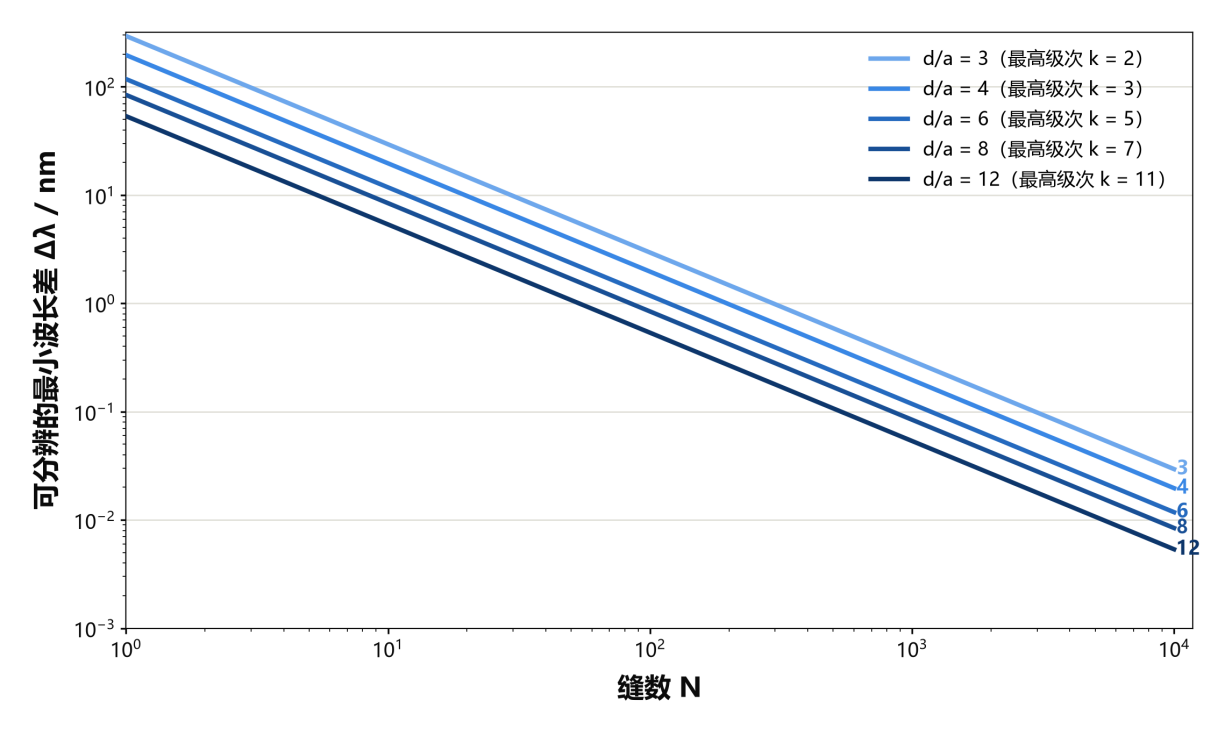
\includegraphics[width=0.9\textwidth]{figures/image19.png}
\caption{可分辨的最小波长差随缝数的变化}
\label{fig:resolving-dlambda}
\end{figure}

\section{衍射现象验证实验}

\subsection{实验目的}

通过实物光学实验，直观验证仿真与理论推导结果，观测单缝衍射、光栅衍射、缺级现象的真实形貌，对比不同光栅参数下条纹粗细、亮度、分辨能力的差异，为视频实拍素材提供真实画面支撑，实现理论、仿真、实验三位一体的科普闭环。

\subsection{实验器材}

氦氖激光器（632.8 nm 单色光源）、精密可调单狭缝、不同刻线密度标准光栅、光学光具座、白色观测光屏、高精度测距尺、游标卡尺。器材精度满足大学物理光学实验标准，可清晰观测各级衍射条纹。

\subsection{实验内容与步骤}

\begin{enumerate}[label={第\arabic*步：}, leftmargin=2.6em, itemsep=2pt]
\item 搭建同轴光学光路，校准激光器、衍射元件、光屏中心对齐，保证入射光垂直入射。
\item 单缝衍射实验：逐步调节狭缝宽度，观测条纹宽窄、亮度变化规律并记录现象。
\item 光栅衍射实验：更换不同光栅常数的光栅，观测规则明亮条纹，验证光栅分光特性。
\item 缺级验证：选用满足整数比值关系的光栅，清晰观测缺级现象，记录缺级级次。
\item 对比分析：对比不同总缝数光栅的谱线精细度，定性验证半角宽度与分辨本领规律。
\end{enumerate}

实验装置如图~\ref{fig:setup}所示。

\begin{figure}[htbp]
\centering
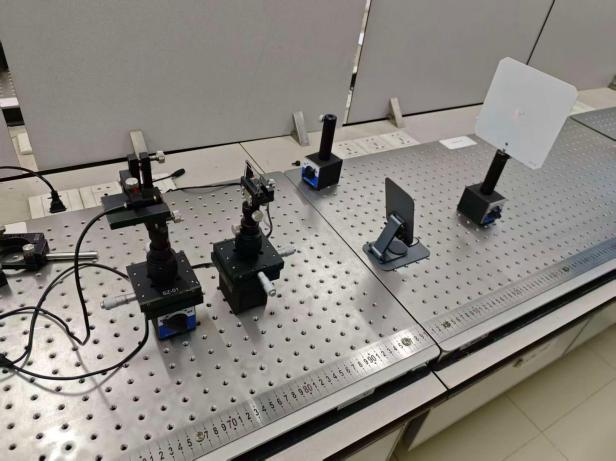
\includegraphics[width=0.9\textwidth]{figures/image20.jpeg}
\caption{实验装置图}
\label{fig:setup}
\end{figure}

\subsection{实验数据与误差分析}

实验记录各组条纹间距、条纹粗细、缺级级次等观测数据，结合理论公式计算理论值，对比实验误差。主要误差来源包括光路同轴度偏差、狭缝边缘衍射干扰、环境杂散光干扰、人眼读数偏差等。通过多次测量取平均值、遮光降噪、精密光路校准等方式降低误差，保证实验结果可靠。不同缝数下观测到的衍射光强分布如图~\ref{fig:diffraction-N}所示，(a)(b)(c)(d)依次对应 $N=1$、$N=2$、$N=5$、$N=100$，可直观看到主极大锐度随缝数增加而提高、半角宽度随之减小的规律。

\begin{figure}[htbp]
\centering
\begin{subfigure}[b]{0.48\textwidth}
\centering
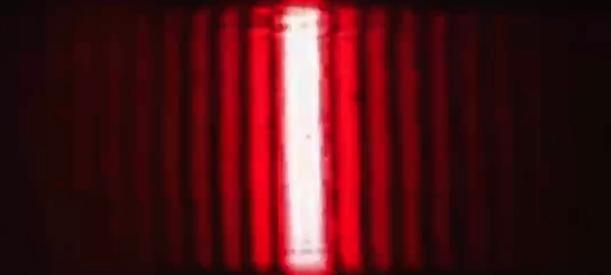
\includegraphics[width=\textwidth]{figures/image21.jpeg}
\caption{$N=1$ 衍射光强分布}
\label{fig:diff-a}
\end{subfigure}
\hfill
\begin{subfigure}[b]{0.48\textwidth}
\centering
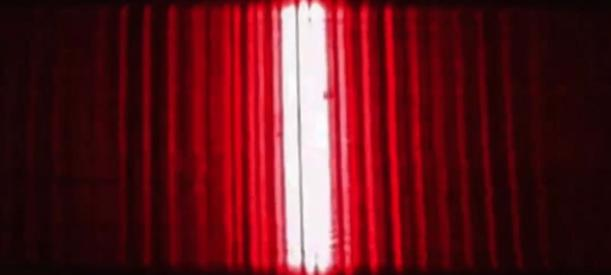
\includegraphics[width=\textwidth]{figures/image22.jpeg}
\caption{$N=2$ 衍射光强分布}
\label{fig:diff-b}
\end{subfigure}
\hfill
\begin{subfigure}[b]{0.48\textwidth}
\centering
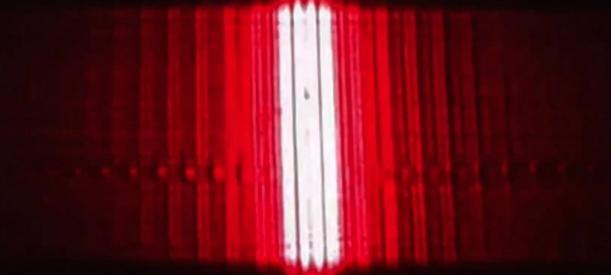
\includegraphics[width=\textwidth]{figures/image23.jpeg}
\caption{$N=5$ 衍射光强分布}
\label{fig:diff-c}
\end{subfigure}
\hfill
\begin{subfigure}[b]{0.48\textwidth}
\centering
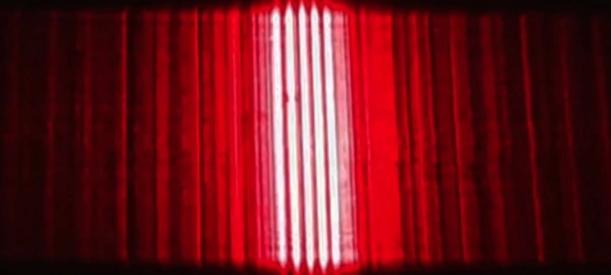
\includegraphics[width=\textwidth]{figures/image24.jpeg}
\caption{$N=100$ 衍射光强分布}
\label{fig:diff-d}
\end{subfigure}

\caption{不同缝数下的衍射光强分布}
\label{fig:diffraction-N}
\end{figure}

\chapter{视频设计与呈现}

\section{视频结构设计}

本科普视频总时长约173秒，整体采用「大国重器悬念引入—科学历史溯源—分层原理拆解—核心特性解析—前沿应用升华—互动体验引流」的递进式叙事结构，节奏张弛有度，兼顾大众观赏性与学术严谨性，适配中小学科普、大学物理辅助教学双重场景。

\subsection{开篇引入：大国重器与光栅价值（15s）}

本段定位为悬念引流、价值铺垫。画面选取ASML光刻机精密光学系统特写、3nm芯片蚀刻微观画面，聚焦大众熟知的高端制造场景，快速建立认知共鸣。通过文案点出光栅“有器无心”的行业痛点，点明光栅是高端光刻机的核心密码，抛出核心问题，引发观众探索兴趣，快速拔高项目立意，将基础光学原理与国家高端制造绑定。整体节奏紧凑、科技感极强，快速抓住观众注意力。

\subsection{历史溯源：夫琅禾费与光栅发展（13s）}

本段完成科学溯源，补齐理论发展脉络。画面采用复古画风，展示夫琅禾费人物肖像、1821年光栅实验线稿，还原光栅理论的诞生背景。通过画面蒙太奇转场，从19世纪基础实验画面平滑过渡到现代光谱仪、光刻机、人造太阳等大国重器画面，串联起“百年科学理论支撑现代顶尖科技”的逻辑，让抽象原理具备历史厚重感与现实价值。

\subsection{原理拆解：从单缝衍射到光栅衍射（62s）}

本段为视频核心教学主体，分为单缝衍射、多缝干涉两个层级递进讲解。以生活中羽毛衍射实拍现象切入，降低入门门槛，再过渡到标准化物理模型。通过二维光路动画、三维光场演化、矢量叠加动态演示，逐帧拆解子波发射、光程差形成、振幅叠加的完整物理过程。同步配套公式分步推导动画，实现画面、配音、公式、物理意义四维同步，让零基础观众能看懂、有基础观众能学透彻，完美解决光学原理抽象难懂的痛点。

\subsection{特性讲解：缺级、半角宽度与分辨本领（58s）}

本段聚焦光栅三大核心特性，层层递进解析光栅高精度分光的本质。通过光强曲线动态叠加动画，直观演示单缝衍射调制、多缝干涉叠加形成缺级的全过程；通过参数动态调节动画，展示总缝数N变化对亮纹半角宽度的影响；依托瑞利判据可视化动画，通俗讲解光谱分辨本领的物理逻辑。所有抽象指标全部转化为肉眼可见的动态对比，知识点逻辑闭环、无断层。

\subsection{应用升华：大国重器中的光栅技术（25s）}

本段实现从理论回归工程、从知识升华价值。画面展示我国郭守敬望远镜LAMOST、羲和号卫星、国产光刻机、人造太阳等自主科研重器，详细对应光栅技术的实际应用场景。文案升华基础科学的重要性，传递“小小光栅，撑起大国精密制造上限”的核心主旨，强化科技自信与科学探索精神，提升视频立意与传播价值。

\subsection{结尾互动：沉浸式体验引导（收尾）}

打破传统科普视频单向输出模式，增加交互式体验闭环。视频结尾展示自主开发的光栅衍射仿真网页，演示实时调节缝宽、缝数、波长参数，动态改变衍射图样的交互效果。屏幕展示专属二维码，引导观众自主上手实验，将被动观看转化为主动探索，延伸科普效果，提升作品创新性与实用性。

\section{制作工具}

本项目全流程采用专业影视、动画、仿真、剪辑、设计工具制作，分工明确、各司其职，保障视频画质精良、原理严谨、观感流畅，全套工具均为行业主流专业软件。

\begin{table}[htbp]
\centering
\begin{tabular}{ll}
\toprule
软件名称 & 具体工作内容 \\
\midrule
剪映专业版 & 全片剪辑、节奏把控、音画同步、画面合成 \\
Blender 5.2.1 & 制作三维光场传播、立体衍射光路、光学设备场景建模 \\
Manim & 二维动画、公式动效 \\
Mathematica & 数值仿真与科学素材生成 \\
HTML & 交互式仿真网页开发 \\
\bottomrule
\end{tabular}
\end{table}

\section{动画实现}

\subsection{三维光场演化动画}

本次实验基于 Blender 平台，以几何节点程序化计算+波纹修改器为核心技术方案，实现光栅衍射的三维光波场动态模拟。将二维接收平面离散为高精度网格，把电场振幅的数值映射为网格顶点的 Z 向位移，以曲面的起伏直观表征光场振幅的空间分布；同时配套理论公式对照与视角动画，分别完成单缝衍射、多缝光栅衍射的三维可视化视频制作。

衍射光场程序化生成基于惠更斯-菲涅耳原理，通过 Blender 几何节点系统实现单缝衍射光场的数值计算：将接收平面离散为高密度网格，逐点计算电场复振幅，将振幅值线性映射为网格顶点的 Z 向位移，生成起伏的三维波场曲面。

场景背景同步配套单缝衍射的理论公式与光强分布曲线。多缝光栅衍射三维模拟通过几何节点实现多缝衍射光场的相干叠加计算：对每条狭缝分别计算单缝衍射场，再引入相邻狭缝间的相位差，将所有狭缝的衍射场相干叠加得到总光场；接收面网格的顶点位移同步反映总电场的振幅分布，曲面上自然呈现出等间距的干涉主极大结构，主极大之间分布着次级极小与次极大，与光栅衍射的理论特征完全吻合。

从三维视角可直观观察到：狭缝数量越多，干涉主极大的形态越锐利，主极大之间的暗区范围越宽，准确复现了多缝衍射条纹的特性。Blender 建模界面与几何节点工作流如图~\ref{fig:blender}所示，(a)为建模界面，(b)为工作流。

\begin{figure}[htbp]
\centering
\begin{subfigure}[b]{0.48\textwidth}
\centering
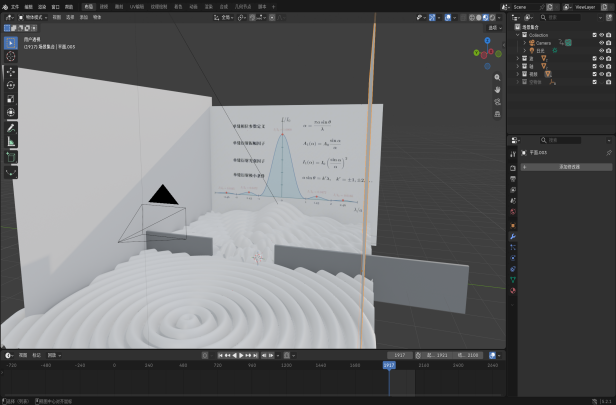
\includegraphics[width=\textwidth]{figures/image25.png}
\caption{Blender建模界面}
\label{fig:blender-a}
\end{subfigure}
\hfill
\begin{subfigure}[b]{0.48\textwidth}
\centering
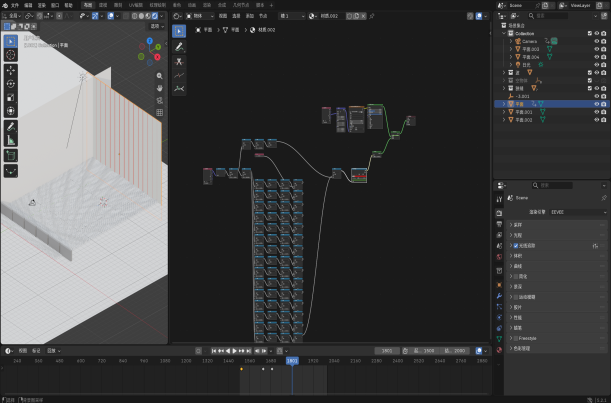
\includegraphics[width=\textwidth]{figures/image26.png}
\caption{Blender工作流}
\label{fig:blender-b}
\end{subfigure}

\caption{Blender 三维光场动画制作}
\label{fig:blender}
\end{figure}

\subsection{二维衍射光路动画}

二维衍射光路动画依托 Manim 动画引擎进行绘制，严格参照大学物理教材标准建立标准化光学光路模型，图形线条规范统一，物理标注严谨准确。动画采用路径描边的逐帧生成方式，动态还原平行光入射狭缝、子波发射、衍射光传播的完整光路过程，动态标注缝宽 $a$、光栅常数 $d$、衍射角 $\theta$、光程差、相位差等关键物理量。

动画使用色彩区分入射光、衍射光以及相干叠加区域，配合矢量箭头直观表现各子波的振动相位变化，将单缝内部子波分解、多缝之间光程差形成的抽象过程可视化。动画节奏与配音讲解完全同步，讲解到对应知识点时同步展示光路变化，规避静态示意图难以表现动态传播过程的短板，适配课堂教学的演示需求。动画效果与代码界面如图~\ref{fig:optical-path}所示，(a)为单缝衍射光路动画效果图，(b)为对应的 Manim 代码界面。

\begin{figure}[htbp]
\centering
\begin{subfigure}[b]{0.48\textwidth}
\centering
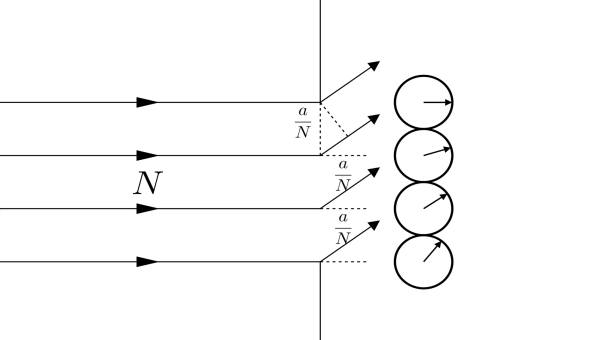
\includegraphics[width=\textwidth]{figures/image27.png}
\caption{单缝衍射光路动画效果图}
\label{fig:path-a}
\end{subfigure}
\hfill
\begin{subfigure}[b]{0.48\textwidth}
\centering
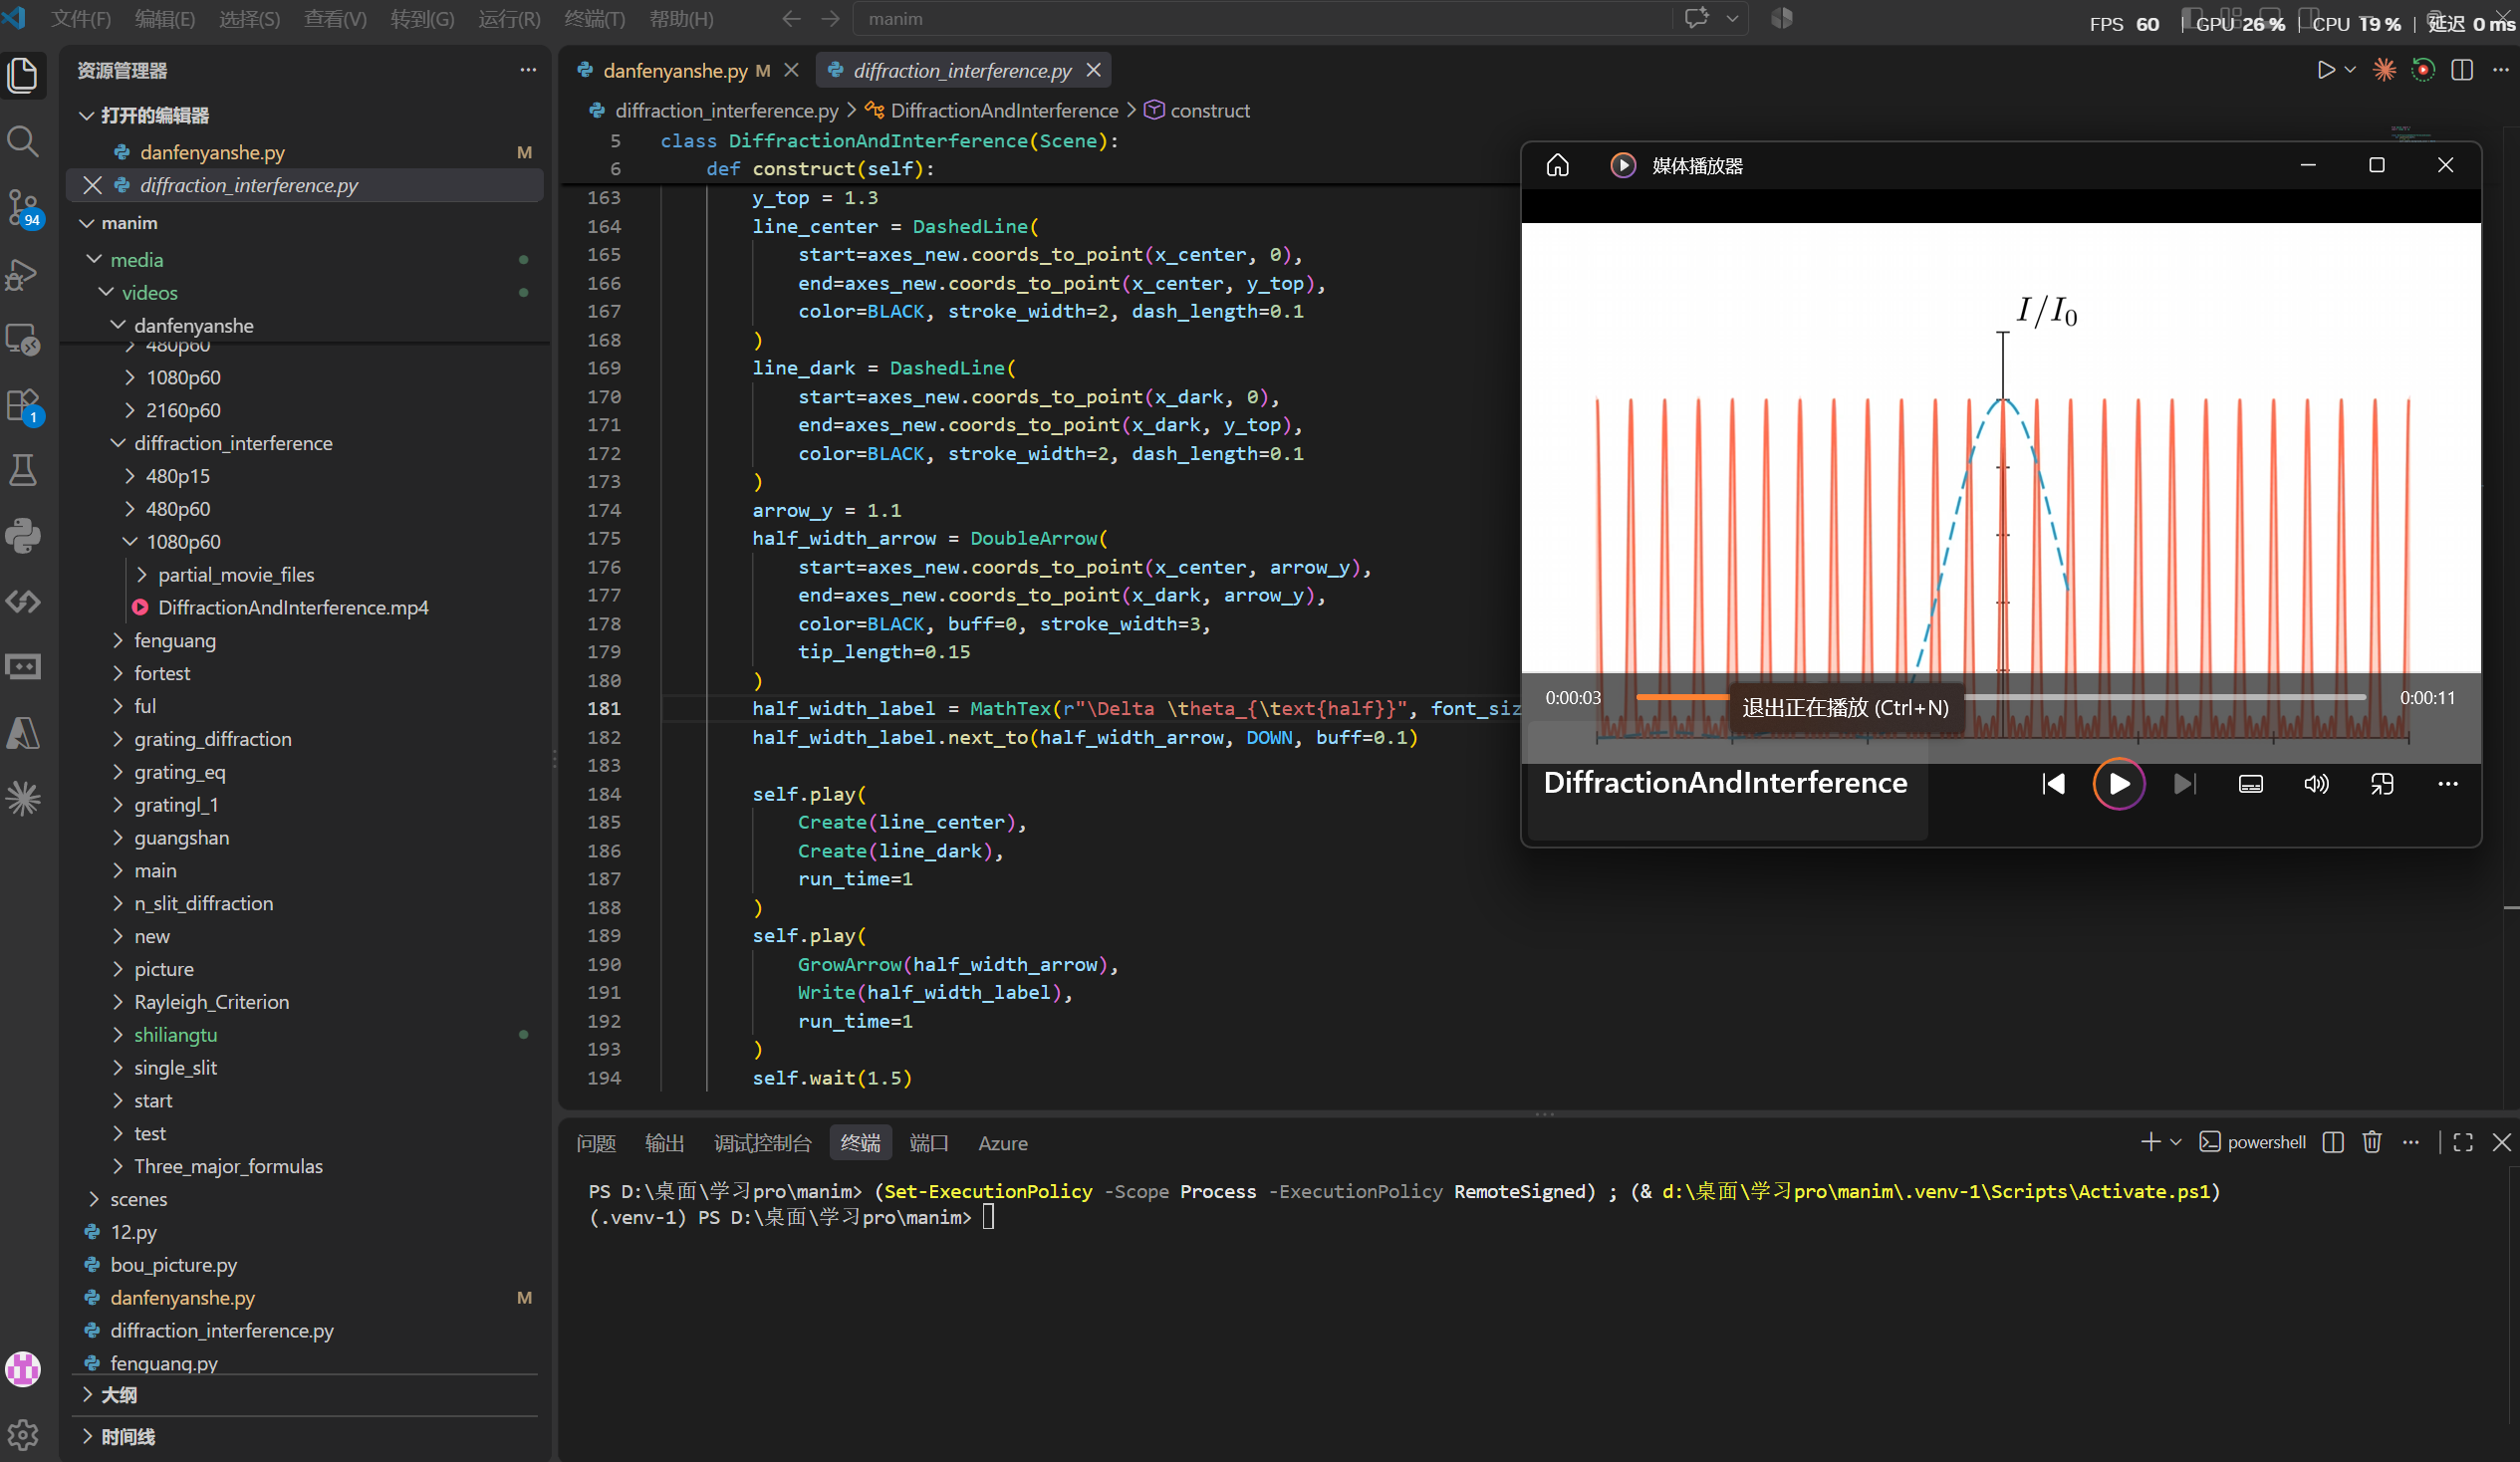
\includegraphics[width=\textwidth]{figures/image28.png}
\caption{单缝衍射光路动画 Manim 代码界面}
\label{fig:path-b}
\end{subfigure}

\caption{二维衍射光路动画}
\label{fig:optical-path}
\end{figure}

\subsection{光强分布动画}

光强分布动画全部采用 Python 数值仿真输出的真实物理数据作为绘制依据，杜绝手绘动画带来的物理失真问题。借助 Manim 实现光强曲线逐点描边的生成动画，依次演示单缝衍射包络、多缝干涉光强曲线，再通过图像变换展示二者相乘得到光栅衍射总光强的完整过程。

针对缺级、半角宽度、色分辨本领等核心特性，设置分屏对照动画，动态修改缝数、光栅常数、缝宽等参数，直观表现参数改变对光强曲线、谱线锐度带来的变化。公式采用分步弹出解析的动画形式，每一项公式出现均对应光强图像的物理变化，例如展示半角宽度时，同步在光强曲线上绘制主极大中心与相邻暗纹的标记虚线、双向箭头与符号标注，将抽象数学符号和光强分布图像一一对应，帮助受众理解公式背后的物理内涵，而不是单纯记忆数学表达式。多缝干涉光强分布效果与代码界面如图~\ref{fig:intensity}所示。

\begin{figure}[htbp]
\centering
\begin{subfigure}[b]{0.48\textwidth}
\centering
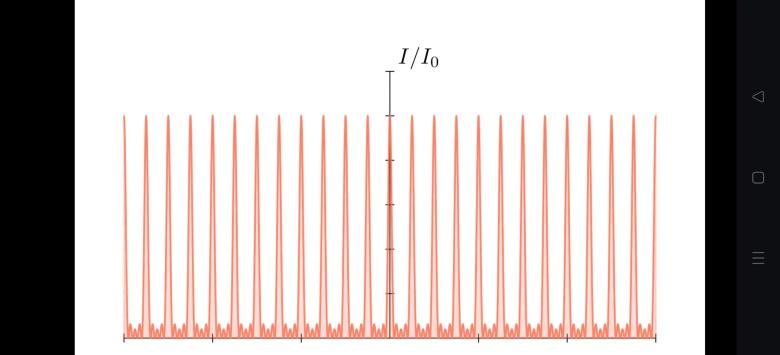
\includegraphics[width=\textwidth]{figures/image29.jpeg}
\caption{多缝干涉光强分布效果图}
\label{fig:inten-a}
\end{subfigure}
\hfill
\begin{subfigure}[b]{0.48\textwidth}
\centering
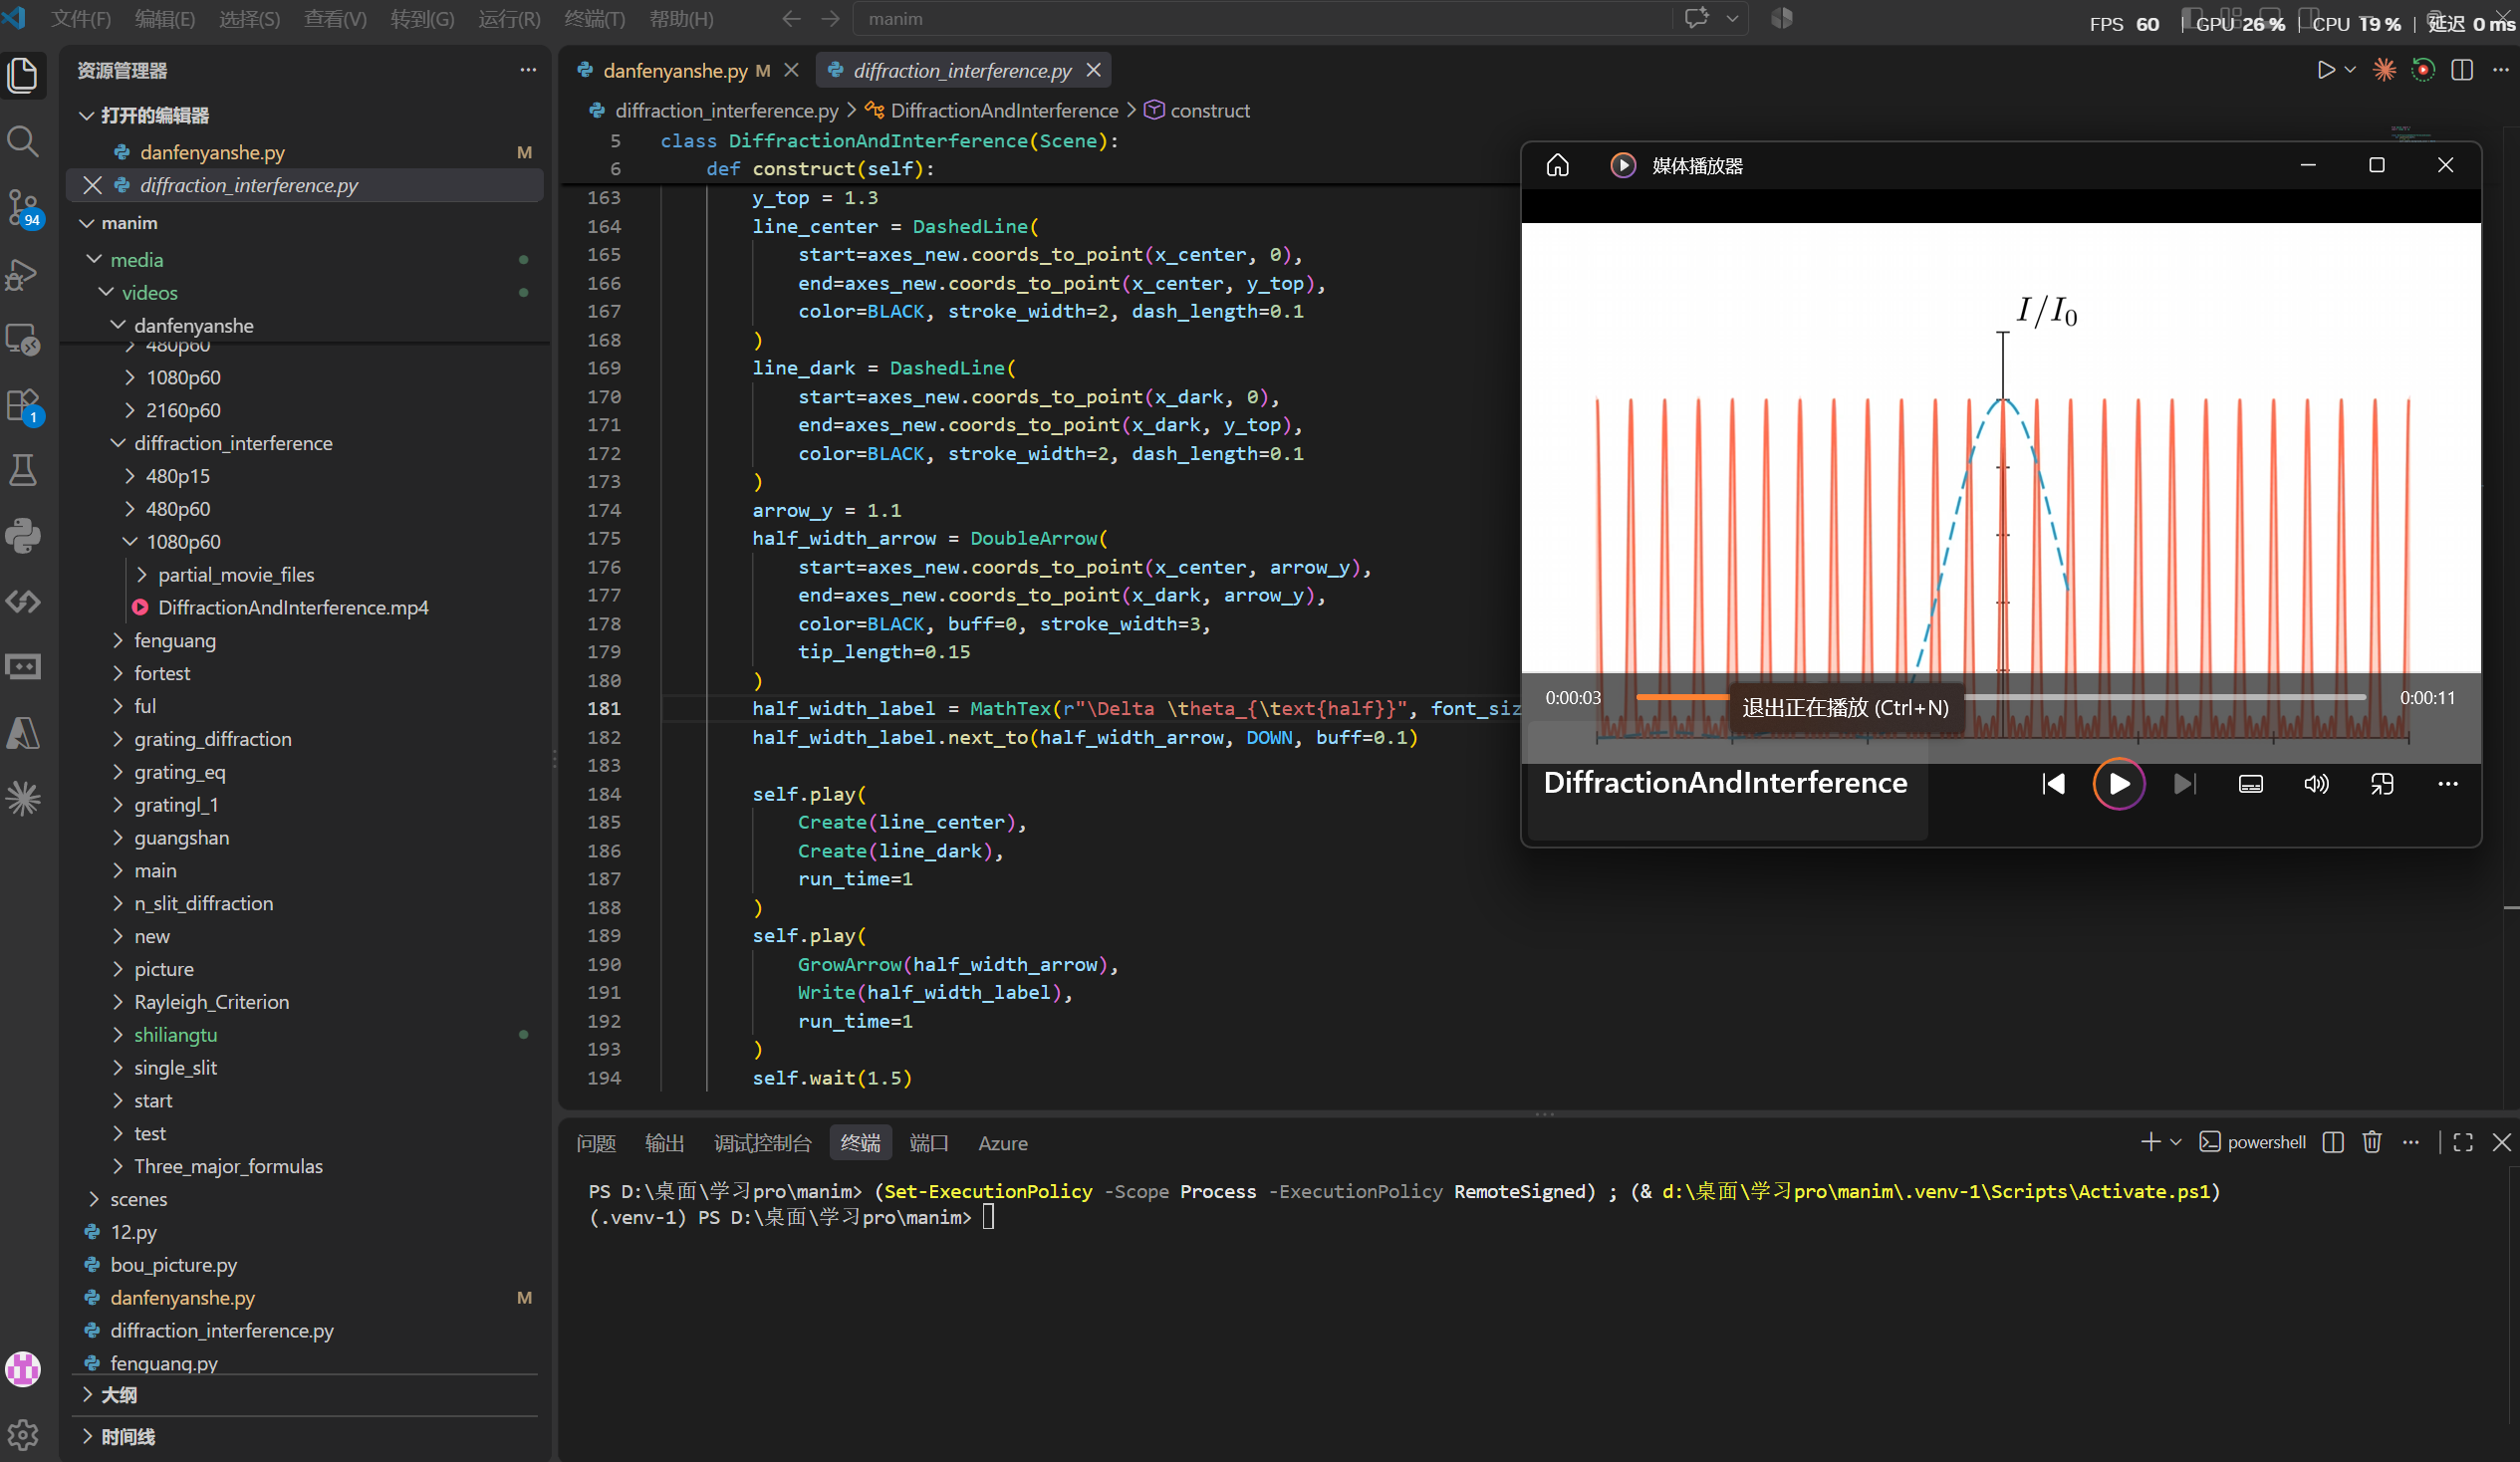
\includegraphics[width=\textwidth]{figures/image28.png}
\caption{多缝干涉光强分布 Manim 代码界面}
\label{fig:inten-b}
\end{subfigure}

\caption{光强分布动画}
\label{fig:intensity}
\end{figure}

\subsection{公式推导动画}

依托仿真真实数据生成光强曲线，采用逐点描边动画动态绘制曲线成型过程，杜绝手绘失真问题。公式采用分步出现、逐项解析的动画逻辑，每一步推导对应对应物理图像。缺级叠加、半角宽度对比、分辨本领变化均采用分屏对照动画，参数变化直观可见，让观众清晰理解公式背后的物理意义，而非死记公式。公式推导动画效果与制作代码界面如图~\ref{fig:formula}所示，(a)为多缝干涉公式效果图，(b)为制作代码界面。

\begin{figure}[htbp]
\centering
\begin{subfigure}[b]{0.48\textwidth}
\centering
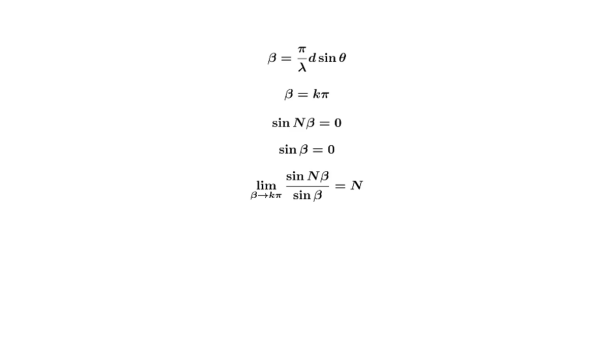
\includegraphics[width=\textwidth]{figures/image30.png}
\caption{多缝干涉公式效果图}
\label{fig:form-a}
\end{subfigure}
\hfill
\begin{subfigure}[b]{0.48\textwidth}
\centering
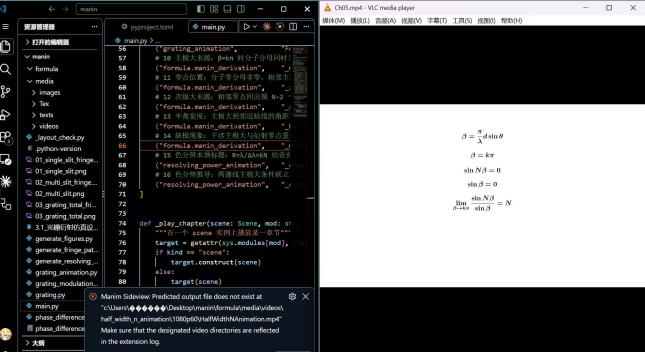
\includegraphics[width=\textwidth]{figures/image31.jpeg}
\caption{多缝干涉公式制作代码界面}
\label{fig:form-b}
\end{subfigure}

\caption{公式推导动画}
\label{fig:formula}
\end{figure}

\subsection{剪辑动画}

光栅衍射历史部分与片尾部分的剪辑界面如图~\ref{fig:editing}所示，(a)为历史部分剪辑界面，(b)为片尾部分剪辑界面。

\begin{figure}[htbp]
\centering
\begin{subfigure}[b]{0.48\textwidth}
\centering
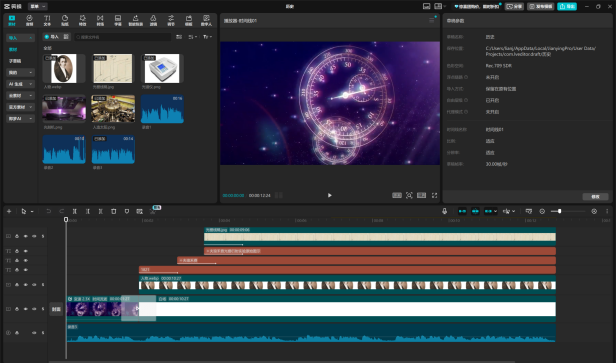
\includegraphics[width=\textwidth]{figures/image32.png}
\caption{光栅衍射历史部分剪辑界面}
\label{fig:edit-a}
\end{subfigure}
\hfill
\begin{subfigure}[b]{0.48\textwidth}
\centering
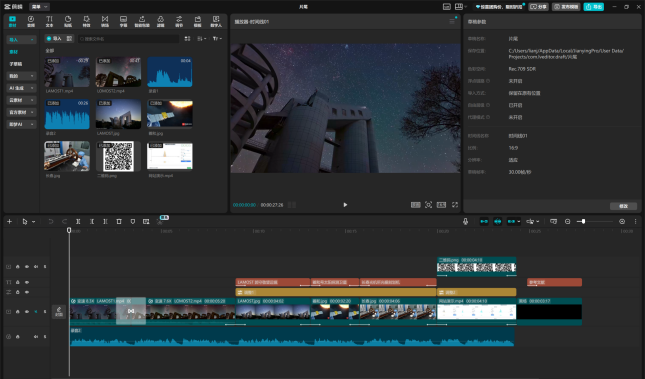
\includegraphics[width=\textwidth]{figures/image33.png}
\caption{光栅衍射片尾部分剪辑界面}
\label{fig:edit-b}
\end{subfigure}

\caption{视频剪辑界面}
\label{fig:editing}
\end{figure}

\section{多媒体素材整合}

\subsection{素材分类与规整}

项目海量素材进行标准化分类管理，分为实拍素材、三维动画素材、二维动效素材、图文字幕素材、音频素材五大类。

实拍素材包含光刻机官方宣传片、LAMOST望远镜延时摄影、羽毛衍射实拍、光学实验实拍；动画素材包含全套光路、矢量叠加、光强曲线、参数变化动画；图文素材包含科学人物画像、设备介绍卡片、公式模板、标题字幕、互动二维码；音频素材包含专业配音、科技转场音效、沉浸式背景配乐。

所有素材统一分辨率、统一色彩规范，便于剪辑整合。剪辑草稿界面如图~\ref{fig:draft}所示。

\begin{figure}[htbp]
\centering
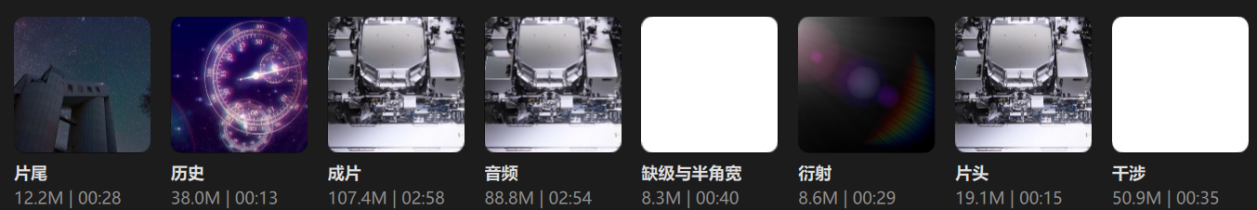
\includegraphics[width=0.9\textwidth]{figures/image34.png}
\caption{剪辑草稿界面}
\label{fig:draft}
\end{figure}

\subsection{剪辑节奏把控}

差异化分段把控视频节奏：开篇与结尾升华段落节奏明快、镜头切换利落，增强视觉冲击力；原理推导、公式讲解、特性分析段落节奏舒缓，延长关键画面停留时间，适配观众理解吸收速度。

转场方式精细化区分，历史段落用淡入淡出、原理递进用元素承接转场、科技展示用快切闪转，整体节奏层次分明、观感舒适。各段配音整合的剪辑界面如图~\ref{fig:dubbing}所示。

\begin{figure}[htbp]
\centering
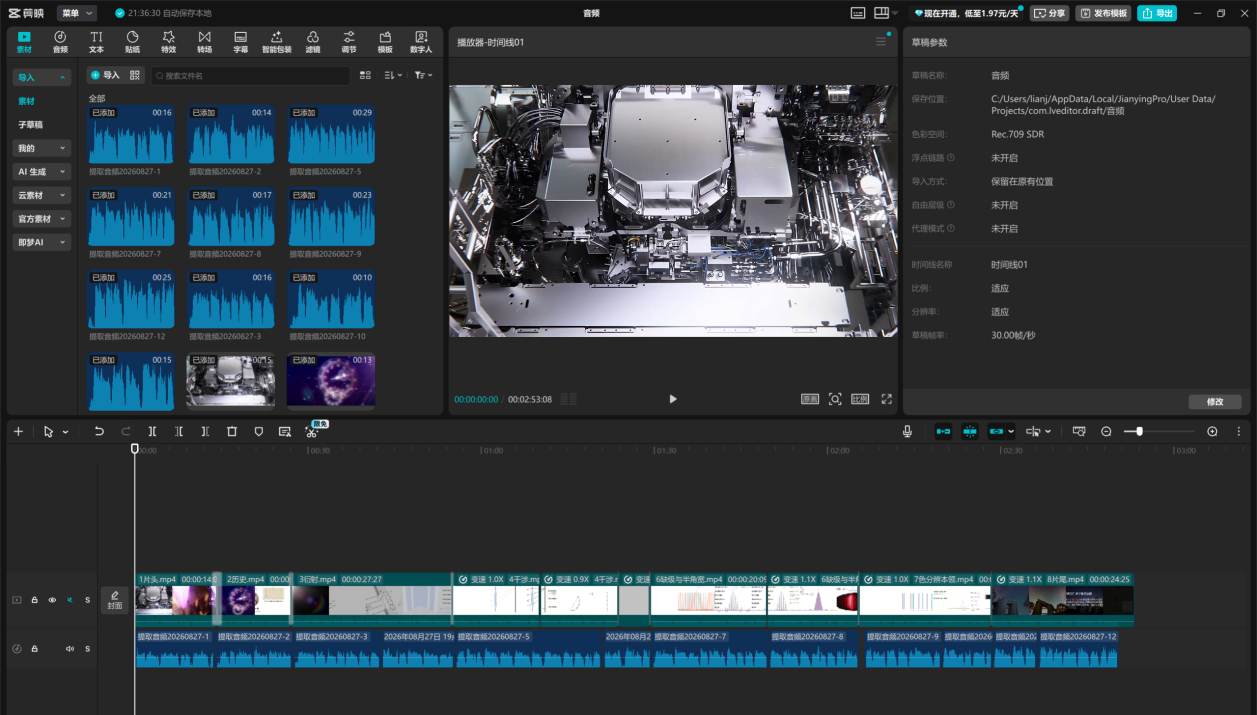
\includegraphics[width=0.9\textwidth]{figures/image35.png}
\caption{汇总各段加配音剪辑界面}
\label{fig:dubbing}
\end{figure}

\subsection{音画同步与包装规范}

实现配音、字幕、动画、音效四维精准同步，关键词、核心结论同步高亮提示。全片统一科技蓝主色调，历史段落复古暖黄、应用段落高亮通透，色彩分区明确。

字幕严格遵循学术规范，物理符号斜体、公式居中、重点结论高亮，画面干净高级、专业性强。全片1080P高清渲染、帧率稳定，画质达到竞赛级作品标准。字幕与背景音乐制作界面如图~\ref{fig:subtitles}所示。

\begin{figure}[htbp]
\centering
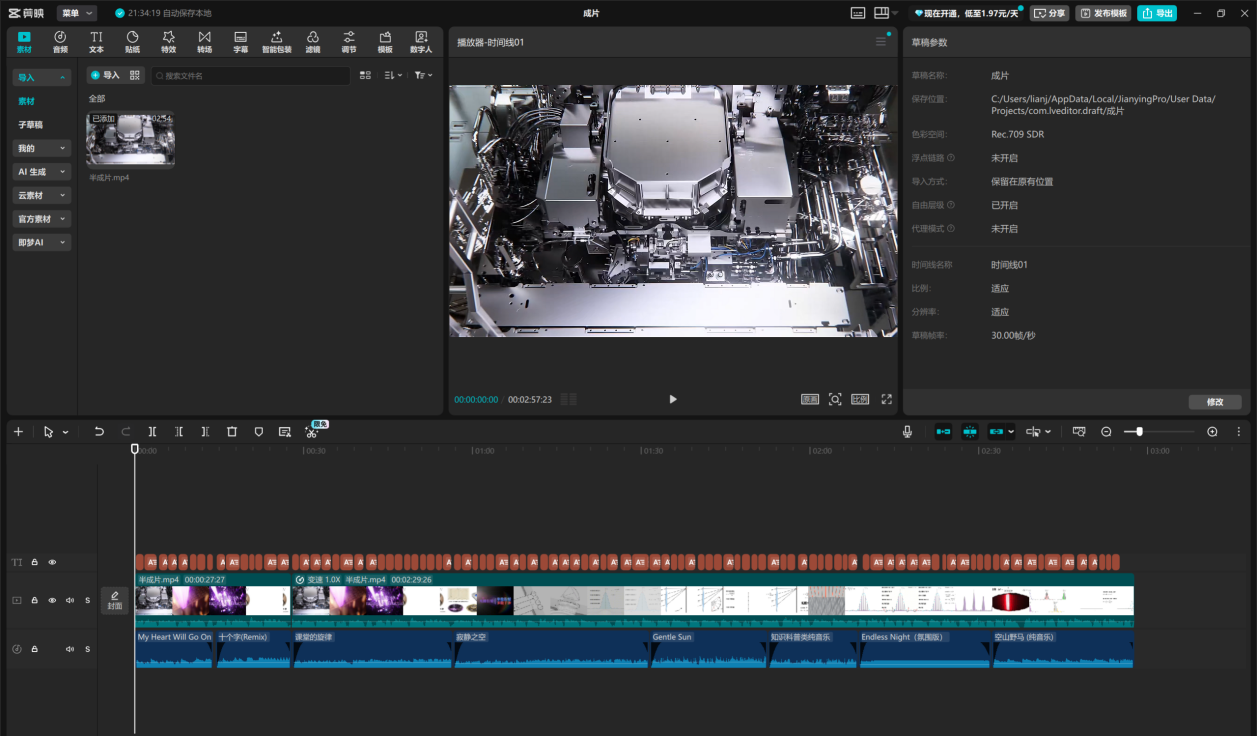
\includegraphics[width=0.9\textwidth]{figures/image36.png}
\caption{加字幕背景音乐剪辑界面}
\label{fig:subtitles}
\end{figure}

\chapter{创新点与总结}

\section{创新点}

\subsection{教学形式创新：科普动画结合前沿重器应用}

突破传统物理科普“重理论、轻应用、无场景”的弊端，将抽象波动光学原理与我国光刻机、巡天望远镜、人造太阳等大国重器深度绑定，让基础物理知识落地到高端科研与工业场景。采用三维立体动画+二维教学动效+真实实拍素材的多元呈现形式，兼顾趣味性、观赏性与学术严谨性，既适合大众科普传播，也可作为高校物理课堂、物理实验的标准化辅助教学资源。

\subsection{内容设计创新：基础原理到工程应用的递进呈现}

内容架构完全遵循人类认知规律，构建「生活现象—科学历史—基础原理—核心特性—工程应用」的完整知识闭环。从具象实拍现象切入，逐层拆解单缝衍射、多缝干涉、光栅衍射、缺级、分辨本领等难点知识点，层层递进、逻辑无断层，完整覆盖大学物理光栅衍射全部考点，同时拓展前沿工程应用，实现“课内知识+课外前沿”的双向拓展，内容深度与适配广度远超普通科普作品。

\subsection{交互设计创新：参数可调的沉浸式衍射体验}

打破传统科普视频单向传播的局限性，配套开发可自主操作的光栅衍射交互网页。观众可手动调节缝宽、光栅常数、总缝数、入射光波长等核心参数，实时观测衍射图样、光强曲线的动态变化，自主验证理论规律。将被动观看升级为主动探究式学习，弥补视频无法个性化演示参数变量的短板，极大提升科普学习效果，具备极强的教学实用价值与创新性。

\section{总结}

本项目完整完成了光栅衍射科普微视频的理论研究、仿真实验、动画制作、剪辑包装、交互开发全流程工作。作品系统梳理了惠更斯-菲涅耳原理、夫琅禾费衍射、单缝衍射、多缝干涉、光栅缺级、半角宽度、色分辨本领的全套理论体系，通过高精度仿真与可视化动画，彻底解决光栅衍射原理抽象、难点难懂的教学痛点。

项目将基础物理理论与国家高端精密制造、前沿天文科研、可控核聚变等大国工程相结合，既普及了专业光学知识，又展现了基础科学对国家科技发展的支撑作用，具备良好的科普价值、教学价值与思政价值。成品视频画面精良、逻辑严谨、节奏舒适、立意深刻，配套交互工具实用性极强，可广泛应用于校园物理教学、线上科普传播、科创竞赛展示等场景。

本次项目实践也积累了光学可视化、科学动画制作、科普内容设计的完整经验，后续可进一步拓展衍射光学、光谱技术等相关科普内容，完善光学科普体系，持续优化交互体验，让基础科学知识以更通俗、更直观、更有趣的形式走进大众与课堂。

\begin{thebibliography}{9}
\addcontentsline{toc}{chapter}{\bibname}
\bibitem{ref1} 赵凯华, 钟锡华. 光学[M]. 北京大学出版社, 2004.
\bibitem{ref2} 梁铨廷. 物理光学[M]. 电子工业出版社, 2012.
\bibitem{ref3} 张三慧. 大学物理学：波动与光学分册[M]. 清华大学出版社, 2019.
\bibitem{ref4} 郁道银, 谈恒英. 工程光学[M]. 机械工业出版社, 2016.
\bibitem{ref5} 中国科学院国家天文台. 郭守敬望远镜（LAMOST）科学成果简介[EB/OL].
\bibitem{ref6} 周炳琨. 激光原理[M]. 国防工业出版社, 2014.
\bibitem{ref7} 约瑟夫·W·古德曼. 傅里叶光学导论[M]. 电子工业出版社, 2020.
\end{thebibliography}

\chapter*{附件1：组员分工}
\addcontentsline{toc}{chapter}{附件1：组员分工}

\begin{table}[htbp]
\centering
\begin{tabular}{ll}
\toprule
成员序号 & 负责模块 \\
\midrule
成员1 & 策划、文案、配音、剪辑、项目报告书 \\
成员2 & 二维图形动画制作 \\
成员3 & 三维动画制作、PPT \\
成员4 & 公式推导动画制作 \\
成员5 & 初步文案思路 \\
\bottomrule
\end{tabular}
\end{table}

\chapter*{附件2：程序代码（外部附件）}
\addcontentsline{toc}{chapter}{附件2：程序代码（外部附件）}

为保证报告正文的紧凑性与可读性，全部 8 个程序源码文件不再内嵌于正文，而以电子附件形式随报告一并提交，存放于「代码附件」目录。各文件功能简述如下：

\begin{table}[htbp]
\centering
\small
\begin{tabular}{lll}
\toprule
文件名 & 类型 & 功能简述 \\
\midrule
danfenyanshe.py & Manim 动画 & 单缝衍射光路动画：入射平行光、单缝绘制、相位圆（矢量）示意、出射光角度变换与光强曲线演示 \\
diffraction\_interference.py & Manim 动画 & 光栅衍射总光强曲线演示：单缝衍射因子与多缝干涉因子相乘、半角宽度标记动画 \\
shiliangtu.py & Manim 动画 & 旋转矢量法动画：$N$ 个振幅矢量首尾相接形成合矢量，演示多缝干涉相位叠加 \\
guangshan.py & Manim 动画 & 光栅衍射光路动画：多缝光栅、入射平行光、波前传播与衍射角标注 \\
single\_slit.py & Manim 动画 & 单缝衍射光强分布曲线、暗纹与明纹位置标注动画 \\
generate\_figures.py & 数值仿真绘图 & 计算并绘制单缝衍射、多缝干涉、光栅总光强归一化曲线（对应图~\ref{fig:sim-output}(a)(c)(e)） \\
generate\_fringe\_patterns.py & 数值仿真绘图 & 由一维光强分布生成二维条纹图样（对应图~\ref{fig:sim-output}(b)(d)(f)） \\
generate\_resolving\_power.py & 数值仿真绘图 & 色分辨本领 $R=kN$、缺级修正及可分辨最小波长差随缝数变化曲线（对应图~\ref{fig:resolving-N}、图~\ref{fig:resolving-missing}、图~\ref{fig:resolving-dlambda}） \\
\bottomrule
\end{tabular}
\end{table}

以光栅衍射总光强的数值计算为例，其核心实现如下（完整源码见「代码附件」目录）：

\begin{lstlisting}[style=pycode]
alpha = np.pi * a * sin_theta / wavelength
beta  = np.pi * d * sin_theta / wavelength
with np.errstate(divide='ignore', invalid='ignore'):
    I_single = np.where(np.abs(alpha) < 1e-12, 1.0,
                        (np.sin(alpha) / alpha) ** 2)     # 单缝衍射因子
    I_multi  = np.where(np.abs(np.sin(beta)) < 1e-12,
                        np.where(np.abs(beta % np.pi) < 1e-12, N**2, 0.0),
                        (np.sin(N * beta) / np.sin(beta)) ** 2)   # 多缝干涉因子
I_total = I_single * I_multi     # 光栅衍射总光强
\end{lstlisting}

\end{document}
